% Este trabalho está licenciado sob a Licença Atribuição-CompartilhaIgual 4.0 Internacional Creative Commons. Para visualizar uma cópia desta licença, visite http://creativecommons.org/licenses/by-sa/4.0/deed.pt_BR ou mande uma carta para Creative Commons, PO Box 1866, Mountain View, CA 94042, USA.

\chapter{Derivação}\label{cap_deriv}

Neste capítulo, estudamos os métodos fundamentais de derivação numérica de funções.

\section{Derivadas de Primeira Ordem}\label{cap_deriv_sec_df}

\hl{A derivada de uma função $f$ num ponto $x$} é, por definição,
\begin{equation}\hleq
  f'(x) := \lim_{h\to 0} \frac{f(x+h) - f(x)}{h}.
\end{equation}
Assim sendo e assumindo $h>0$\footnote{Para fixar notação, assumiremos $h>0$ ao longo deste capítulo.} próximo de zero, temos que \hl{$f'(x)$ pode ser aproximada pela \emph{fórmula de diferenças finitas}}
\begin{subequations}\label{cap_deriv_sec_df:eq:fdf}\hleq
  \begin{align}
    f'(x) &\approx \frac{f(x+h) - f(x)}{h}\\
          &=: D_hf(x).
  \end{align}
\end{subequations}
Geometricamente, isto é análogo a aproximar a declividade da reta tangente ao gráfico da função $f$ no ponto $(x, f(x))$ pela declividade da reta secante ao gráfico da função $f$ pelos pontos $(x, f(x))$ e $(x+h, f(x+h))$ (consulte a Figura~\ref{cap_deriv_sec_df:fig:intro_deriv}).

\begin{figure}[H]
  \centering
  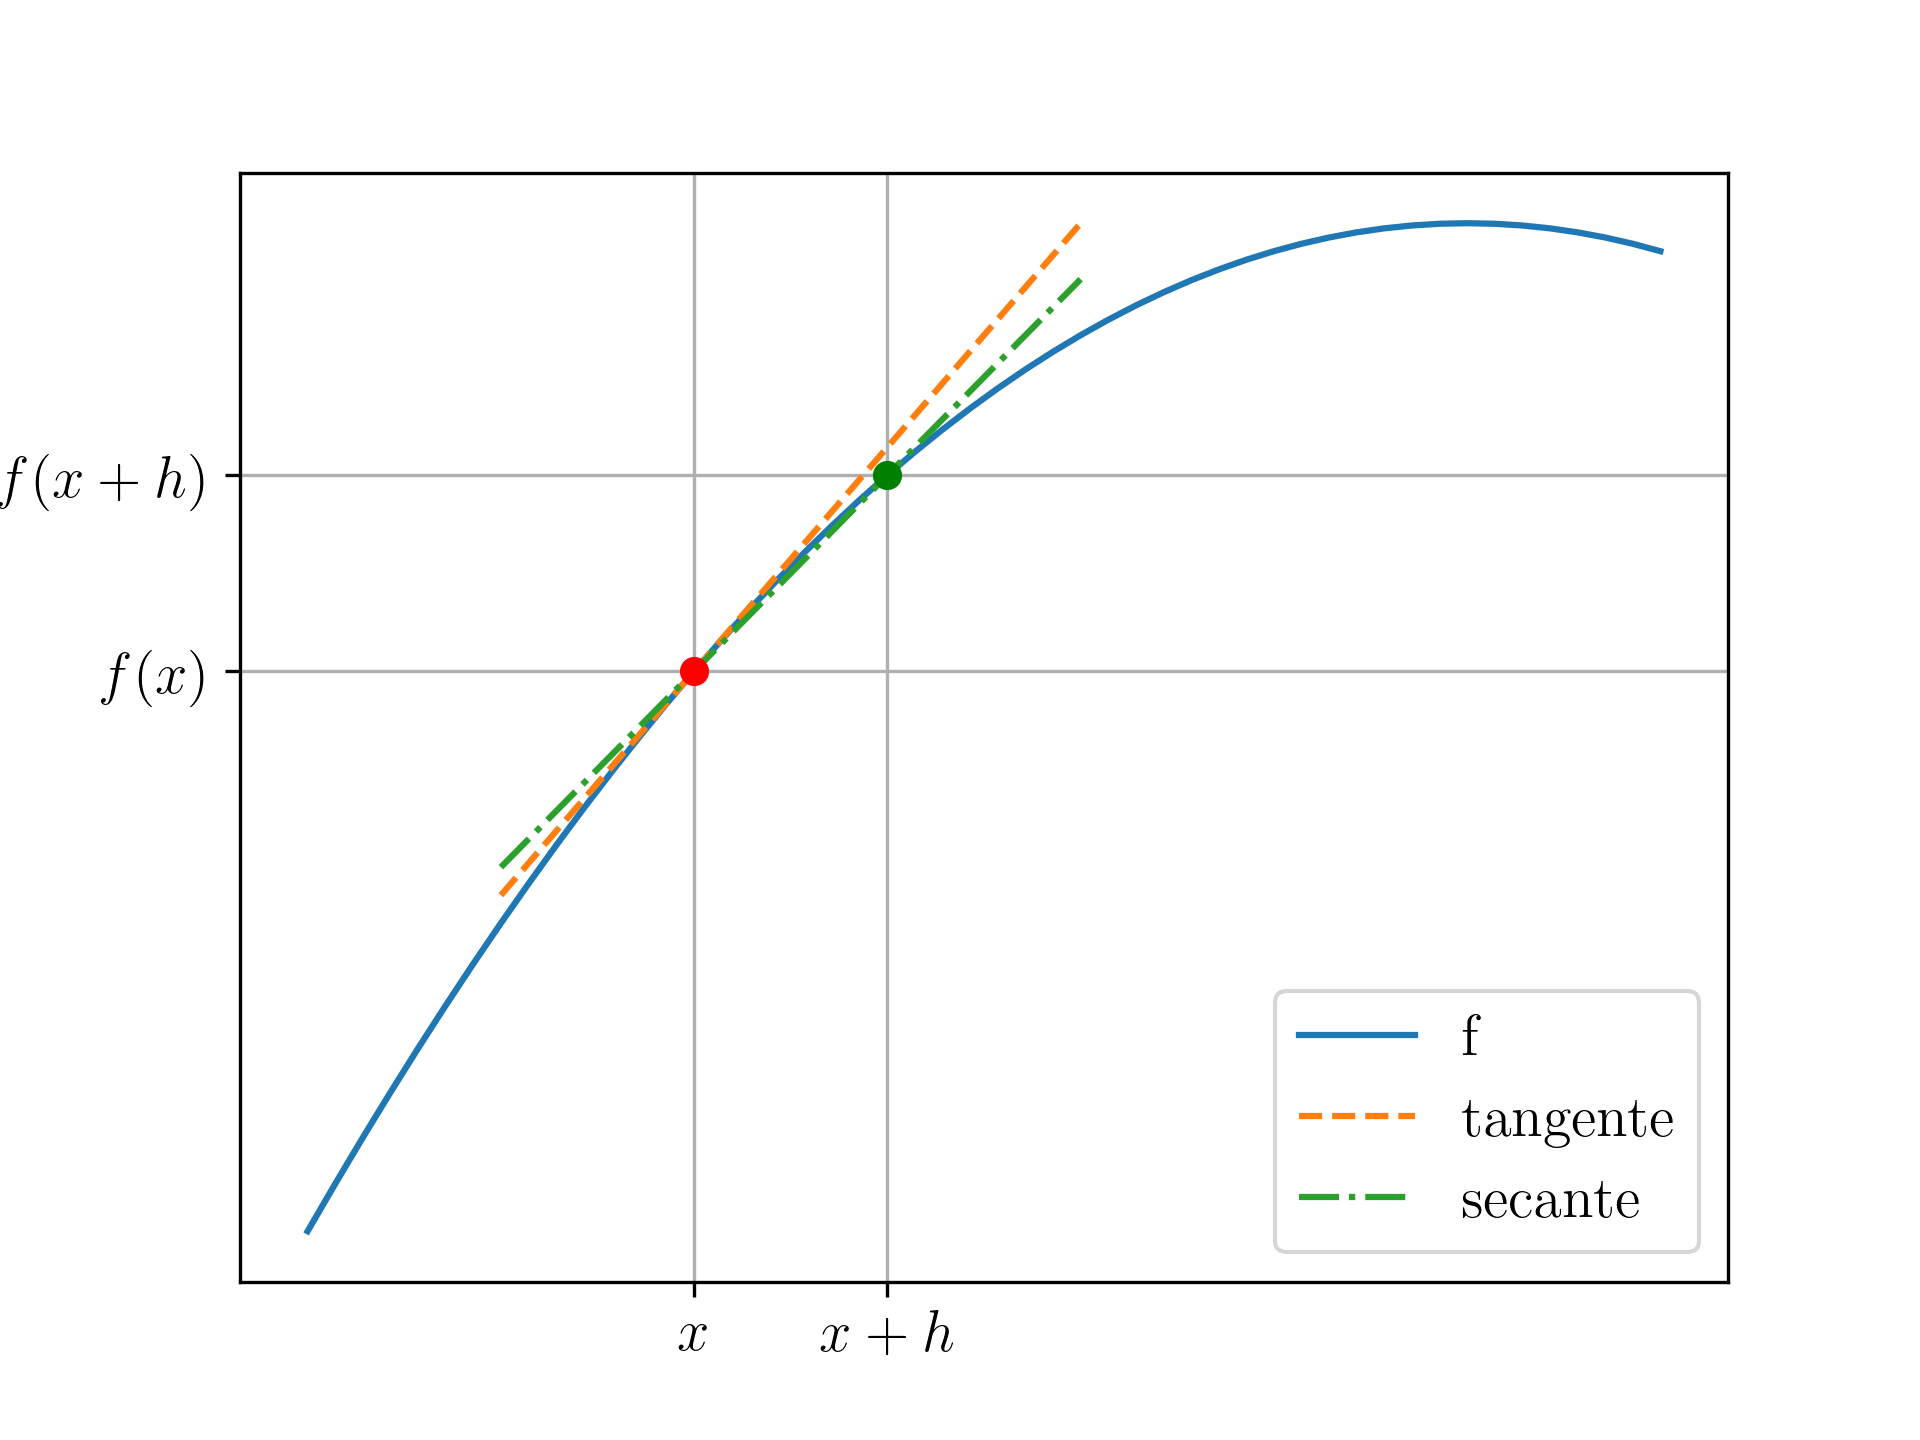
\includegraphics[width=0.8\textwidth]{cap_deriv/dados/fig_intro_deriv/fig}
  \caption{Interpretação geométrica da aproximação da derivada pela razão fundamental.}
  \label{cap_deriv_sec_df:fig:intro_deriv}
\end{figure}

\begin{ex}\label{cap_deriv_sec_df:ex_intro_deriv}
  A derivada de $f(x) = \sen(x)$ no ponto $\pi/3$ é $f'(\pi/3) = \cos(\pi/3)=0.5$. Agora, usando a aproximação pela fórmula de diferenças finitas~\eqref{cap_deriv_sec_df:eq:fdf}, temos
  \begin{subequations}
    \begin{align}
      f'\left(\frac{\pi}{3}\right) &\approx D_hf\left(\frac{\pi}{3}\right) \\
                                   &= \frac{f\left(\frac{\pi}{3}+h\right)-f\left(\frac{\pi}{3}\right)}{h}\\
                                   &= \frac{\sen\left(\frac{\pi}{3}+h\right)-\sen\left(\frac{\pi}{3}\right)}{h}. 
    \end{align}
\end{subequations}
Na Tabela~\ref{cap_deriv_sec_df:tab:ex_intro_deriv} temos os valores desta aproximação para diferentes escolhas da passo $h$.

\begin{table}[H]
  \centering
  \caption{Valores aproximados da derivada de $f(x)=\sen(x)$ no ponto $x=\pi/3$ usado a fórmula de diferenças finitas \eqref{cap_deriv_sec_df:eq:fdf}.}
  \begin{tabular}{l|c}
    $h$ & $Df(\pi/3)$ \\ \hline
    $10^{-1}$ & $4.55902\E-1$ \\
    $10^{-2}$ & $4.95662\E-1$ \\
    $10^{-3}$ & $4.99567\E-1$ \\
    $10^{-5}$ & $4.99996\E-1$ \\
    $10^{-7}$ & $5.00000\E-1$ \\
    $10^{-10}$ & $5.00000\E-1$ \\\hline
  \end{tabular}
  \label{cap_deriv_sec_df:tab:ex_intro_deriv}
\end{table}

\begin{lstlisting}
import numpy as np

def dfdx(f, x, h=1e-7):
    df = (f(x+h) - f(x))/h
    return df

f = lambda x: np.sin(x)
x = np.pi/3
h = 1e-7
dfdx = dfdx(f, x, h)
\end{lstlisting}
\end{ex}

\subsection{Diferenças Finitas por Polinômio de Taylor}

Vamos estudar o desenvolvimento de \emph{fórmulas de diferenças finitas} via polinômios de Taylor.

\subsubsection{Fórmula de Diferenças Finitas Progressiva de Ordem $h$}

A aproximação por polinômio de Taylor de grau 1 de uma dada função $f$ em torno no ponto $x$ é
\begin{equation}\label{cap_deriv_sec_df:eq:poli_Taylor_grau_1}
  f(x+h) = f(x) + hf'(x) + O(h^2).
\end{equation}
Isolando $f'(x)$, obtemos
\begin{equation}
  f'(x) = \frac{f(x+h) - f(x)}{h} + O(h).
\end{equation}
Isto nos fornece a chamada \hl{\emph{fórmula de diferenças finitas progressiva de ordem $h$}}
\begin{equation}\label{cap_deriv_sec_df:eq:dfp_h}\hleq
  D_{+,h}f(x) := \frac{f(x+h) - f(x)}{h}.
\end{equation}
Observemos que \hl{a ordem da fórmula se refere a do \emph{erro de truncamento} com respeito ao passo $h$}.

\begin{ex}\label{cap_deriv_sec_df:ex:dfp_h}
  Consideremos o problema de aproximar a derivada da função $f(x) = \sen(x)$ no ponto $\pi/3$. Usando a fórmula de diferenças finitas progressiva de ordem $h$ obtemos
  \begin{subequations}
    \begin{align}
      f'\left(\frac{\pi}{3}\right) &\approx D_{+,h}f(x)\\
      &= \frac{f\left(\frac{\pi}{3}+h\right)-f\left(\frac{\pi}{3}\right)}{h}\\
      &= \frac{\sen\left(\frac{\pi}{3}+h\right)-\sen\left(\frac{\pi}{3}\right)}{h}. 
    \end{align}
\end{subequations}
Na Tabela~\ref{cap_deriv_sec_df:tab:ex_dfp_h} temos os valores desta aproximação para diferentes escolhas de $h$, bem como, o erro absoluto da aproximação de $f'(\pi/3)$ por $D_{+,h}f(\pi/3)$.

\begin{table}[h!]
  \centering
  \caption{Resultados referente ao Exemplo~\ref{cap_deriv_sec_df:ex:dfp_h}.}
  \begin{tabular}{l|c|c}
    $h$ & $D_{+,h}f(\pi/3)$ & $|f'(\pi/3)-D_{+,h}f(\pi/3)|$\\ \hline
    $10^{-1}$ & $4.55902\E-1$ & $4.4\E-2$ \\
    $10^{-2}$ & $4.95662\E-1$ & $4.3\E-3$ \\
    $10^{-3}$ & $4.99567\E-1$ & $4.3\E-4$ \\
    $10^{-5}$ & $4.99996\E-1$ & $4.3\E-6$ \\
    $10^{-10}$ & $5.00000\E-1$ & $4.1\E-8$ \\\hline
  \end{tabular}
  \label{cap_deriv_sec_df:tab:ex_dfp_h}
\end{table}

\begin{lstlisting}[caption=dfp\_h.py]
import numpy as np

def dfp_h(f, x, h=1e-7):
    df = (f(x+h) - f(x))/h
    return df

f = lambda x: np.sin(x)
x = np.pi/3
h = 1e-1
dfdx = dfp_h(f, x, h)
\end{lstlisting}
\end{ex}

\begin{obs}\normalfont{(\hl{Erro de Truncamento}.)}
  No Exemplo \ref{cap_deriv_sec_df:ex:dfp_h}, podemos observar que o erro absoluto na aproximação de $f'(x)$ por $D_{+,h}f(x)$ decresce conforme a ordem do erro de truncamento para valores moderados de $h$ (consulte a Tabela~\ref{cap_deriv_sec_df:tab:ex_dfp_h}). Agora, para valores de $h$ muito pequenos (por exemplo, $h=10^{-10}$), o erro $|f'(x)-D_{+,h}f(x)|$ não segue mais a tendência de decaimento na mesma ordem do de truncamento. Isto se deve a dominância dos erros de arredondamento para valores muito pequenos de $h$.
\end{obs}

\subsubsection{Fórmula de Diferenças Finitas Regressiva de Ordem $h$}

Substituindo $h$ por $-h$ no polinômio de Taylor de grau 1 \eqref{cap_deriv_sec_df:eq:poli_Taylor_grau_1}, temos
\begin{equation}
  f(x-h) = f(x) - hf'(x) + O(h^2),
\end{equation}
donde obtemos a \hl{\emph{fórmula de diferenças finitas regressiva de ordem $h$}}
\begin{equation}\label{cap_deriv_sec_df:eq:dfr_h}\hleq
  D_{-,h}f(x) := \frac{f(x) - f(x-h)}{h}.
\end{equation}

\begin{ex}\label{cap_deriv_sec_df:ex:dfr_h}
  Consideremos o problema de aproximar a derivada da função $f(x) = \sen(x)$ no ponto $\pi/3$. Usando a fórmula de diferenças finitas regressiva de ordem $h$ obtemos
  \begin{subequations}
    \begin{align}
      f'\left(\frac{\pi}{3}\right) &\approx D_{-,h}f(x) \\
                                   &= \frac{f\left(\frac{\pi}{3}\right)-f\left(\frac{\pi}{3}-h\right)}{h}\\
                                   &= \frac{\sen\left(\frac{\pi}{3}\right)-\sen\left(\frac{\pi}{3}-h\right)}{h}. 
    \end{align}
  \end{subequations}
Na Tabela~\ref{cap_deriv_sec_df:tab:ex_dfr_h} temos os valores desta aproximação para diferentes escolhas de $h$, bem como, o erro absoluto da aproximação de $f'(\pi/3)$ por $D_{-,h}f(\pi/3)$.

\begin{table}[h!]
  \centering
  \caption{Resultados referente ao Exemplo~\ref{cap_deriv_sec_df:ex:dfr_h}.}
  \begin{tabular}{l|c|c}
    $h$ & $D_{-,h}f(\pi/3)$ & $|f'(\pi/3)-D_{-,h}f(\pi/3)|$\\ \hline
    $10^{-1}$ & $5.42432\E-1$ & $4.2\E-2$ \\
    $10^{-2}$ & $5.04322\E-1$ & $4.3\E-3$ \\
    $10^{-3}$ & $5.00433\E-1$ & $4.3\E-4$ \\
    $10^{-5}$ & $5.00004\E-1$ & $4.3\E-6$ \\
    $10^{-10}$ & $5.00000\E-1$ & $4.1\E-8$ \\\hline
  \end{tabular}
  \label{cap_deriv_sec_df:tab:ex_dfr_h}
\end{table}

\begin{lstlisting}[caption=dfr\_h.py]
import numpy as np

def dfr_h(f, x, h=1e-7):
    df = (f(x) - f(x-h))/h
    return df

f = lambda x: np.sin(x)
x = np.pi/3
h = 1e-1
dfdx = dfr_h(f, x, h)
\end{lstlisting}
\end{ex}

\subsubsection{Fórumla de Diferenças Finitas Central de Ordem $h^2$}

Usando o polinômio de Taylor de grau 2 para aproximar a função $f(x)$ em torno de $x$, temos
\begin{align}
  f(x+h) &= f(x) + hf'(x) + \frac{h}{2}f''(x) + O(h^3)\\
  f(x-h) &= f(x) - hf'(x) + \frac{h}{2}f''(x) + O(h^3).
\end{align}
Então, subtraindo esta segunda equação da primeira, temos
\begin{equation}
  f(x+h)-f(x-h) = 2hf'(x) + O(h^3).
\end{equation}
Então, isolando $f(x)$, obtemos
\begin{equation}
  f'(x) = \frac{f(x+h)-f(x-h)}{2h} + O(h^2),
\end{equation}
Isto nos fornece a chamada \hl{\emph{fórmula de diferenças finitas central de ordem $h^2$}}
\begin{equation}\label{cap_deriv_sec_df:eq:dfc_h2}\hleq
  D_{0,h^2}f(x) := \frac{f(x+h)-f(x-h)}{2h}.
\end{equation}

\begin{ex}\label{cap_deriv_sec_df:ex:dfc_h2}
  Consideremos o problema de aproximar a derivada da função $f(x) = \sen(x)$ no ponto $\pi/3$. Usando a fórmula de diferenças finitas central de ordem $h^2$ obtemos
  \begin{subequations}
    \begin{align}
      f'\left(\frac{\pi}{3}\right) &\approx D_{0,h^2}f(x) \\
                                   &= \frac{f\left(\frac{\pi}{3}+h\right)-f\left(\frac{\pi}{3}-h\right)}{2h}\\
                                   &= \frac{\sen\left(\frac{\pi}{3}+h\right)-\sen\left(\frac{\pi}{3}-h\right)}{2h}. 
  \end{align}
\end{subequations}
Na Tabela~\ref{cap_deriv_sec_df:tab:ex_dfc_h2} temos os valores desta aproximação para diferentes escolhas de $h$, bem como, o erro absoluto da aproximação de $f'(\pi/3)$ por $D_{0,h^2}f(\pi/3)$.

\begin{table}[h!]
  \centering
  \caption{Resultados referente ao Exemplo~\ref{cap_deriv_sec_df:ex:dfc_h2}.}
  \begin{tabular}{l|c|c}
    $h$ & $D_{0,h^2}f(\pi/3)$ & $|f'(\pi/3)-D_{0,h^2}f(\pi/3)|$\\ \hline
    $10^{-1}$ & $4.99167\E-1$ & $8.3\E-04$ \\
    $10^{-2}$ & $4.99992\E-1$ & $8.3\E-06$ \\
    $10^{-3}$ & $5.00000\E-1$ & $8.3\E-08$ \\
    $10^{-5}$ & $5.00000\E-1$ & $8.3\E-10$ \\
    $10^{-10}$ & $5.00000\E-1$ & $7.8\E-12$ \\\hline
  \end{tabular}
  \label{cap_deriv_sec_df:tab:ex_dfc_h2}
\end{table}


\begin{lstlisting}[caption=dfc\_h2.py]
import numpy as np

def dfc_h2(f, x, h=1e-7):
    df = (f(x+h) - f(x-h))/(2*h)
    return df

f = lambda x: np.sin(x)
x = np.pi/3
h = 1e-1
dfdx = dfc_h2(f, x, h)
\end{lstlisting}
\end{ex}

\subsection*{Exercícios}

\begin{exer}
  Considere a função $f(x) = \cos(x)$. Use a fórmula de diferenças finitas progressiva de ordem $h$ para computar a aproximação de $f'(\pi/3)$ com 5 dígitos significativos corretos.
\end{exer}
\begin{resp}
  $f'(\pi/3) = -0.866025\E+0, h=10^{-7}$
\end{resp}

\begin{exer}
  Considere a função $f(x) = \cos(x)$. Use a fórmula de diferenças finitas regressiva de ordem $h$ para computar a aproximação de $f'(\pi/3)$ com 5 dígitos significativos corretos.
\end{exer}
\begin{resp}
  $f'(\pi/3) = -0.866025\E+0, h=10^{-6}$
\end{resp}

\begin{exer}
  Considere a função $f(x) = \cos(x)$. Use a fórmula de diferenças finitas central de ordem $h^2$ para computar a aproximação de $f'(\pi/3)$ com 5 dígitos significativos corretos.
\end{exer}
\begin{resp}
  $f'(\pi/3) = -0.866025\E+0, h=10^{-3}$
\end{resp}

\begin{exer}\label{cap_deriv_sec_df:exer:df_fun}
  Calcule aproximações da derivada de
  \begin{equation}
    f(x) = \frac{\sen(x+2) - e^{-x^2}}{x^2 + \ln(x+2)}+x
  \end{equation}
no ponto $x=2.5$ dadas pelas seguintes fórmulas de diferenças finitas com $h=10^{-2}$:
\begin{enumerate}[a)]
\item progressiva de ordem $h$.
\item regressiva de ordem $h$.
\item central de ordem $h^2$.
\end{enumerate}
\end{exer}
\begin{resp}
  a)~$D_{+,h}f(2.5)=1,05949$; b)~$D_{-,h}f(2.5)=1,05877$; c)~$D_{0,h^2}f(2.5)=1,05913$;
\end{resp}

\begin{exer}\label{cap_deriv_sec_df:exer:df_tab}
  Considere a seguinte tabela de pontos
  \begin{center}
    \begin{tabular}{l|rr}
      $i$ & $x_i$ & $y_i$\\\hline
      $1$ & $2.0$ & $1.86$\\
      $2$ & $2.1$ & $1.90$\\
      $3$ & $2.2$ & $2.01$\\
      $4$ & $2.3$ & $2.16$\\
      $5$ & $2.4$ & $2.23$\\
      $6$ & $2.5$ & $2.31$\\\hline
    \end{tabular}
  \end{center}
Calcule aproximações de $dy/dx$ usando diferenças finitas centrais de ordem $h^2$ quando possível e, caso contrário, diferenças finitas progressiva ou regressiva conforme o caso.
\end{exer}
\begin{resp}
  \begin{center}
    \begin{tabular}{l|r}
      $i$ & $dy/dx$\\\hline
      $1$ & $4.0\E-2$\\
      $2$ & $7.5\E-1$\\
      $3$ & $1.3\E+0$\\
      $4$ & $1.1\E+0$\\
      $5$ & $7.5\E-1$\\
      $6$ & $8.0\E-1$\\\hline
    \end{tabular}
  \end{center}
\end{resp}

\begin{exer}
  Use uma combinação de polinômios de Taylor de grau 2 para desenvolver a fórmula de diferenças finitas progressiva de ordem $h^2$
  \begin{equation}\label{cap_deriv_sec_df:eq:dfp_h2}
    D_{+,h^2}(x) := \frac{1}{2h}\left[-3f(x) + 4f(x+h) - f(x+2h)\right].
  \end{equation}
  Então, aplique-a para computar $f'(\pi/3)$ com $f(x)=\sen(x)$ e verifique o comportamento do erro $|D_{+,h^2}(\pi/3) - f'(\pi/3)|$ em relação à ordem de truncamento da fórmula.
\end{exer}

\begin{exer}
  Use uma combinação de polinômios de Taylor de grau 2 para desenvolver a fórmula de diferenças finitas regressiva de ordem $h^2$
  \begin{equation}\label{cap_deriv_sec_df:eq:dfr_h2}
    D_{-,h^2}(x) := \frac{1}{2h}\left[3f(x) - 4f(x-h) + f(x-2h)\right].
  \end{equation}
  Então, aplique-a para computar $f'(\pi/3)$ com $f(x)=\sen(x)$ e verifique o comportamento do erro $|D_{+,h^2}(\pi/3) - f'(\pi/3)|$ em relação à ordem de truncamento da fórmula.
\end{exer}

\begin{exer}
  Refaça as computações do Exercício \ref{cap_deriv_sec_df:exer:df_tab} usando fórmulas de diferenças finitas de ordem $h^2$ para todos os pontos.
\end{exer}
\begin{resp}
  \begin{center}
    \begin{tabular}{l|r}
      $i$ & $dy/dx$\\\hline
      $1$ & $5.0\E-2$\\
      $2$ & $7.5\E-1$\\
      $3$ & $1.3\E+0$\\
      $4$ & $1.1\E+0$\\
      $5$ & $7.5\E-1$\\
      $6$ & $8.5\E-1$\\\hline
    \end{tabular}
  \end{center}  
\end{resp}

\section{Derivadas de Segunda Ordem}\label{cap_deriv_sec_d2f}

Diferentemente do usual em técnicas analíticas, no âmbito da matemática numérica é preferível obter aproximações diretas de derivadas de segunda ordem, em vez de utilizar aproximações sucessivas de derivadas. Na sequência, desenvolvemos e aplicaremos uma fórmula de diferenças finitas central para a aproximação de derivadas de segunda ordem.

Consideremos os seguintes polinômios de Taylor{\taylor} de grau 3 de $f(x)$ em torno do ponto x
\begin{align}
  f(x+h) &= f(x) + hf'(x) + \frac{h^2}{2}f''(x) + \frac{h^3}{3!}f'''(x) + O(h^4),\\
  f(x-h) &= f(x) - hf'(x) + \frac{h^2}{2}f''(x) - \frac{h^3}{3!}f'''(x) + O(h^4).\\
\end{align}
Somando estas duas equações, obtemos
\begin{equation}
  f(x+h)+f(x-h) = 2f(x) + h^2f''(x) + O(h^4).
\end{equation}
Então, isolando $f''(x)$ temos
\begin{equation}
  f''(x) = \frac{f(x+h) - 2f(x) + f(x-h)}{h^2} + \hleq{O(h^2)}.
\end{equation}
Isto nos leva a definição da \hl{\emph{fórmula de diferenças finitas de ordem $h^2$ para a derivada segunda}}
\begin{equation}\hleq
  D^2_{0,h^2} f(x) := \frac{f(x+h) - 2f(x) + f(x-h)}{h^2}.
\end{equation}

\begin{ex}\label{cap_deriv_sec_d2f:ex:d2fc_h2}
  Consideramos o problema de computar a derivada segunda de $f(x) = x^2 + \sen x$ no ponto $x=\pi/6$. Analiticamente, $f''(\pi/6) = 2 - \sen(\pi/6) = 1,5$. Numericamente, vamos explorar as seguintes duas aproximações:
  \begin{enumerate}
  \item[a)] Aplicação de sucessivas diferenças finitas centrais de ordem $h^2$ para derivada primeira, i.e.
    \begin{subequations}\label{cap_deriv_sec_d2f:eq:ddf}
      \begin{align}
        f''(x) &\approx D_{0,h^2}D_{0,h^2}f(x) \\
               &= \frac{D_{0,h^2}f(x+h) - D_{0,h^2}f(x-h)}{2h}
      \end{align}
    \end{subequations}
  \item[b)] Aplicação da fórmula de diferenças finitas central de ordem $h^2$ para a derivada segunda, i.e.
    \begin{subequations}
      \begin{align}
        f''(x) &\approx D_{0,h^2}^2 f(x)\\
               &= \frac{f(x+h) - 2f(x) + f(x-h)}{h^2}.
      \end{align}
    \end{subequations}
  \end{enumerate}

\begin{table}[h!]
  \centering
  \caption{Resultados referente ao Exemplo~\ref{cap_deriv_sec_d2f:ex:d2fc_h2}. Notação: $\delta_{DD}:=|f''(\pi/6)-D_{0,h^2}D_{0,h^2}f(\pi/6)|$ e $\delta_{D^2}:=|f''(\pi/6)-D^2_{0,h^2}f(\pi/6)|$.}
  \begin{tabular}{l|cc|cc}
    $h$ & $D_{0,h^2}D_{0,h^2}f(\pi/6)$ & $\delta_{DD}$ & $D^2_{0,h^2}f(\pi/6)$ & $\delta_{D^2}$ \\ \hline
    $10^{-1}$ &  $1.50166$ & $1.7\E-03$ & $1.50042$ & $4.2\E-04$ \\
    $10^{-2}$ &  $1.50002$ & $1.7\E-05$ & $1.50000$ & $4.2\E-06$ \\
    $10^{-3}$ &  $1.50000$ & $1.7\E-07$ & $1.50000$ & $4.2\E-08$ \\
    $10^{-5}$ &  $1.50000$ & $1.2\E-07$ & $1.50000$ & $1.2\E-07$ \\\hline
  \end{tabular}
  \label{cap_deriv_sec_d2f:tab:ex_d2fc_h2}
\end{table}

Na Tabela~\ref{cap_deriv_sec_d2f:tab:ex_d2fc_h2} temos os valores computados em ambos os casos e seus respectivos erros absolutos para diversas escolhas de $h$. Observamos que a aplicação da diferença finita $D^2_{0,h^2}$ fornece resultados mais precisos (para valores moderados de $h$) do que as sucessivas aplicações de $D_{0,h^2}$. De fato, uma rápida inspeção de \eqref{cap_deriv_sec_d2f:eq:ddf} mostra que
\begin{equation}
  D_{0,h^2}D_{0,h^2}f(x) = \underbrace{\frac{f(x+2h) - 2f(x) + f(x-2h)}{4h^2}}_{D^2_{0,(2h)^2}f(x)}.
\end{equation}

\begin{lstlisting}[caption=d2fc\_h2.py]
import numpy as np

def d2fc_h2(f, x, h=1e-7):
    df = (f(x+h) - 2*f(x) + f(x-h))/h**2
    return df

f = lambda x: x**2 + np.sin(x)
x = np.pi/6
h = 1e-1
d2fdx2 = d2fc_h2(f, x, h)
print(f'{h}: d2fdx2 = {d2fdx2:.5e}, erro = {np.fabs(d2fdx2-1.5):.1e}')
\end{lstlisting}
\end{ex}

\subsection*{Exercícios}

\begin{exer}\label{exer:d2fc_fun}
  Use a fórmula de diferenças finitas central de ordem $h^2$ para computar aproximações da segunda derivada de
  \begin{equation}
    f(x) = \frac{\sen(x+2) - e^{-x^2}}{x^2 + \ln(x+2)}+x
  \end{equation}
no ponto $x=2,5$. Para tanto, use os passos
\begin{enumerate}[a)]
\item $h=10^{-1}$
\item $h=10^{-2}$
\item $h=10^{-3}$
\item $h=10^{-4}$
\end{enumerate}
Por fim, com base nos resultados obtidos, qual foi o maior passo que forneceu a aproximação com precisão de pelo menos $5$ dígitos significativos? Justifique sua resposta.
\end{exer}
\begin{resp}
  a)~$7.25162\E-2$; b)~$7.24701\E-2$; c)~$7.24696\E-2$; d)~$7.24696\E-2$; $h=10^{-2}$;
\end{resp}

\begin{exer}
  Considere a função $f(x) = e^x\ln(x+1) - x$. Use a fórmula de diferenças finitas central de ordem $h^2$ para computar a aproximação de $f''(1)$ com 6 dígitos significativos corretos.
\end{exer}
\begin{resp}
  $f''(1) = 3.92288\E+0$, $h=10^{-3}$.
\end{resp}


\begin{exer}\label{exer:d2fc_tab}
  Considere a seguinte tabela de pontos
  \begin{center}
    \begin{tabular}{l|cccccc}
      $i$ & $1$ & $2$ & $3$ & $4$ & $5$ & $6$ \\\hline
      $x_i$ & $2,0$ & $2,1$ & $2,2$ & $2,3$ & $2,4$ & $2,5$ \\
      $y_i$ & $1,86$ & $1,90$ & $2,01$ & $2,16$ & $2,23$ & $2,31$ \\\hline
    \end{tabular}
  \end{center}
Calcule a aproximação $d^2y/dx^2$ no ponto $x=2,2$ usando a fórmula de diferenças finitas central de ordem $h^2$.
\end{exer}
\begin{resp}
  $4.0$; 
\end{resp}


\section{Diferenças Finitas por Polinômios Interpoladores}\label{cap_deriv_sec_df_pi}

Vamos estudar como obter \hl{fórmulas de diferenças finitas por polinômios interpoladores}. Seja \hl{$p(x)$ o \emph{polinômio interpolador} dos pontos $\{(x_i,f(x_i))\}_{i=1}^{n+1}$} de uma dada função $f(x)$, com $x_1 < x_2 < \cdots < x_{n+1}$. Então, pelo teorema de Lagrange temos
\begin{equation}\hleq
  f(x) = p(x) + R_{n+1}(x),
\end{equation}
onde \hl{$R(x)$ é o erro na aproximação de $f(x)$ por $p(x)$} e tem a forma
\begin{equation}\hleq
  R_{n+1}(x) = \frac{f^{(n+1)}(\xi)}{(n+1)!}\prod_{j=1}^{n+1}(x-x_j).
\end{equation}
onde $\xi = \xi(x)$.

Deste modo, \hl{a ideia para obtermos as fórmulas de diferenças é aproximarmos $f'(x)$ por $p'(x)$}. Entretanto, isto nos coloca a questão de estimarmos o erro $|f'(x) - p'(x)|$. Por sorte temos os seguinte teorema.

\begin{teo}\label{cap_deriv_sec_df_pi:teo:erro_de_Lagrange_deriv}
  Seja $p(x)$ o polinômio interpolador de uma dada função $f(x)$ pelo pontos $\{(x_i, f(x_i))\}_{i=1}^{n+1}$, com $x_1<x_2<\cdots<x_{n+1}$. Se $f(x)$ é $(n+1)$ continuamente diferenciável, então o resíduo $R_{n+1}^{(k)}(x) = f^{(k)}(x) - p^{(k)}(x)$ é
  \begin{equation}
    R_{n+1}^{(k)} = \frac{f^{(n+1)}(\eta) }{(n+1-k)!}\prod_{j=1}^{n+1-k}(x-\xi_j),
  \end{equation}
onde $\xi_j$ é um ponto tal que $x_j < \xi_j < x_{j+k}$, $j=1, 2, \dotsc, n+1+k$, e $\eta = \eta(x)$ é algum ponto no intervalo de extremos $x$ e $\xi_j$. 
\end{teo}
\begin{dem}
  Veja \cite[Ch.6, Sec.5]{Isaacson1994a}.
\end{dem}

\subsection{Fórmulas de dois pontos}

Para obtermos \hl{fórmulas de diferenças finitas de dois pontos consideramos  $p(x)$ o polinômio interpolador de Lagrange de $f(x)$ pelos pontos $(x_1, f(x_1))$ e $(x_2, f(x_2))$}, com $x_1 < x_2$, i.e.
\begin{align}
  f(x) &= p(x) + R_{2}(x)\\
  &= f(x_1)\frac{x-x_2}{x_1-x_2} + f(x_2)\frac{x-x_1}{x_2-x_1} + R_2(x).
\end{align}
Denotando $h=x_2-x_1$, temos
\begin{equation}
  f(x) = f(x_1)\frac{x-x_2}{-h} + f(x_2)\frac{x-x_1}{h} + R_2(x).
\end{equation}
e, derivando com respeito a $x$
\begin{equation}
  f'(x) = \frac{f(x_2)-f(x_1)}{h} + R_2^{(1)}(x),
\end{equation}
onde $ R_2^{(1)}(x)$ é dado conforme o Teorema~\ref{cap_deriv_sec_df_pi:teo:erro_de_Lagrange_deriv}.

Agora, escolhendo $x=x_1$, temos $x_2 = x_1 + h = x + h$ e, obtemos a \hl{\emph{fórmula de diferenças finitas progressiva de ordem $h$}}
\begin{equation}\hleq
  f(x) = \underbrace{\frac{f(x+h) - f(x)}{h}}_{D_{+,h}f(x)} + O(h).
\end{equation}

Se escolhermos $x=x_2$, temos $x_1 = x_2 - h = x - h$, obtemos a \hl{\emph{fórmula de diferenças finitas regressiva de ordem $h$}}
\begin{equation}\hleq
  f(x) = \underbrace{\frac{f(x) - f(x-h)}{h}}_{D_{-,h}f(x)} + O(h).
\end{equation}

\subsubsection{Fórmulas de três pontos}

Para obtermos \hl{fórmulas de diferenças finitas de três pontos consideramos o polinômio interpolador de Lagrange de $f(x)$ pelos pontos $(x_1, f(x_1))$, $(x_2, f(x_2))$ e $(x_3, f(x_3))$, $x_1<x_2<x_3$}, i.e.
\begin{align}
  f(x) &= f(x_1)\frac{(x-x_2)(x-x_3)}{(x_1-x_2)(x_1-x_3)} \\
  &+ f(x_2)\frac{(x-x_1)(x-x_3)}{(x_2-x_1)(x_2-x_3)} \\
  &+ f(x_3)\frac{(x-x_1)(x-x_2)}{(x_3-x_1)(x_3-x_2)} + R_3(x).
\end{align}
Derivando em relação a $x$, obtemos
\begin{align}\label{eq:aux_deriv1}
  f'(x) &= f{\left (x_{1} \right )}\frac{\left(x_{2} - x_{3}\right) \left(2 x- x_{2} - x_{3}\right)}{\left(x_{1} - x_{2}\right) \left(x_{1} - x_{3}\right) \left(x_{2} - x_{3}\right)} \\
  &+ f{\left (x_{2} \right )}\frac{\left(x_{1} - x_{3}\right) \left(- 2 x + x_{1} + x_{3}\right)}{\left(x_{1} - x_{2}\right) \left(x_{1} - x_{3}\right) \left(x_{2} - x_{3}\right)}\\
  &+ f\left(x_{3} \right)\frac{\left(x_{1} - x_{2}\right)\left(2 x - x_{1} - x_{2}\right)}{\left(x_{1} - x_{2}\right) \left(x_{1} - x_{3}\right) \left(x_{2} - x_{3}\right)} + R_3^{(1)}(x).
\end{align}

Aqui, \hl{podemos escolher por obter fórmulas de diferenças com passo constante ou não}. Por exemplo, denotando $h_1=x_2-x_1$ e $h_2=x_3-x_2$ e escolhendo $x=x_1$, temos $x_2 = x+h_1$ e $x_3 = x+h_1+h_2$. Fazendo estas substituições na expressão acima, obtemos seguinte fórmula de diferenças finitas progressiva
\begin{align}
  D_{+,h1,h2}f(x) &= \frac{1}{h_{1} h_{2} \left(h_{1} + h_{2}\right)} \left(- h_{2} \left(2 h_{1} + h_{2}\right) f{\left (x \right )} \right.\\
    &+ \left. \left(h_{1} + h_{2}\right)^{2} f{\left (x + h_{1} \right )} \right.\\
    &- \left. h_{1}^{2} f{\left (x + h_{1} + h_{2} \right )} \right).
\end{align}
Agora, \hl{assumindo um passo constante $h=h_1=h_2$, obtemos a \emph{fórmula de diferenças progressiva de ordem $h^2$}}
\begin{equation}\hleq
  D_{+,h^2}f(x) = \frac{1}{2 h} \left[- 3 f{\left (x \right )} + 4 f{\left (x + h \right )} - f{\left (x + 2 h \right )}\right].\label{eq:dfp_3pts}
\end{equation}

\hl{Escolhendo $x=x_2$, $x_1=x-h$ e $x_3=x+h$ na equação~{\eqref{eq:aux_deriv1}}, obtemos a \emph{fórmula de diferenças finitas central de ordem $h^2$}}
\begin{equation}\hleq
  D_{0,h^2} = \frac{1}{2 h} \left[f{\left (x + h \right )} - f{\left (x - h \right )}\right].
\end{equation}

Por fim, \hl{escolhendo $x=x_3$, $x_1=x-2h$ e $x_2=x-h$ na equação~{\eqref{eq:aux_deriv1}}, obtemos a \emph{fórmula de diferenças finitas regressiva de ordem $h^2$}}
\begin{equation}\hleq
  D_{-,h^2} = \frac{1}{2 h} \left[3 f{\left (x \right )} - 4 f{\left (x - h \right )}  + f{\left (x - 2 h\right )}\right].
\end{equation}

\subsection{Fórmulas de cinco pontos}

Aqui, \hl{usamos o polinômio interpolador de Lagrange da função $f(x)$ pelos pontos $(x_1, f(x_1)$, $(x_2, f(x_2))$, $(x_3, f(x_3))$ e $(x_5, f(x_5))$}, com $x_1 < x_2 < x_3 < x_4 < x_5$. Isto nos fornece
\begin{equation}
  f(x) = \sum_{i=1}^5 f(x_i)\left(\prod_{j=1, j\neq i}^{5} \frac{x-x_j}{x_i-x_j}\right) + R_5(x).
\end{equation}
Calculando a derivada em relação a $x$, temos
\begin{equation}\label{eq:aux_deriv2}
  f'(x) = \sum_{i=1}^5 f(x_i)\left(\sum_{\overset{j=1}{j\neq i}}^5\prod_{\overset{k=1}{k\neq i, k\neq j}}^{5} \frac{x-x_k}{x_i-x_k}\right) + R^{(1)}_5(x).
\end{equation}

Por exemplo, \hl{substituindo $x_1=x-2h$, $x_2=x-h$, $x_3=x$, $x_4=x+h$ e $x_5=x+2h$} na equação acima, \hl{\emph{obtemos fórmula de diferenças finitas central de ordem $h^4$}}
\begin{equation}\label{eq:dfc_5pts}\hleq
  \begin{aligned}
    D_{+,h^4}f(x) &:= \frac{1}{12h} \left[f{\left (x - 2 h\right )} - 8 f{\left(x - h \right )} \right. \\
    &+ \left. 8 f{\left (x + h \right )} - f{\left (x + 2 h \right )}\right].
  \end{aligned}
\end{equation}

\subsection*{Exercícios}

\begin{exer}\label{exer:dfch4_fun}
  Use a fórmula de diferenças finitas central de ordem $h^4$ para computar a aproximação da derivada de
  \begin{equation}
    f(x) = \frac{\sen(x+2) - e^{-x^2}}{x^2 + \ln(x+2)}+x
  \end{equation}
no ponto $x=2,5$ com passo $h=0,1$.
\end{exer}
\begin{resp}
  $1.05913$
\end{resp}

\begin{exer}\label{exer:df_5pts_pi}
  Obtenha as seguintes fórmulas de diferenças finitas de $5$ pontos com passo $h$ constante e com:
  \begin{enumerate}
  \item[a)] $4$ pontos para frente.
  \item[b)] $1$ ponto para traz e $3$ pontos para frente.
  \item[c)] $2$ pontos para traz e $2$ pontos para frente.
  \item[d)] $3$ pontos para traz e $1$ pontos para frente.
  \item[e)] $4$ pontos para traz.
  \end{enumerate}
\end{exer}
\begin{resp}
  \begin{tiny}
    \begin{align*}
      \text{a)}&~\frac{1}{12 h} \left[3 f{\left (x- 4h \right )} - 16 f{\left (x- 3 h \right )} + 36 f{\left (x- 2 h \right )} - 48 f{\left (x- h \right ) + 25 f{\left (x \right )}}\right]\\
      \text{b)}&~\frac{1}{12 h} \left[- f{\left (x- 3 h \right )} + 6 f{\left ( x- 2 h \right )} - 18 f{\left (x- h \right )} + 10 f{\left (x \right )} + 3 f{\left (x+h \right )}\right]\\
      \text{c)}&~\frac{1}{12h} \left[f{\left (x - 2 h\right )} - 8 f{\left(x - h \right )} + 8 f{\left (x + h \right )} - f{\left (x + 2 h \right )}\right]\\
      \text{d)}&~\frac{1}{12 h} \left[- 3 f{\left ( x-h \right )} - 10 f{\left (x \right )} + 18 f{\left (x+h \right )} - 6 f{\left (x+2 h \right )} + f{\left ( x+3 h \right )}\right]\\
      \text{d)}&~\frac{1}{12 h} \left[- 25 f{\left (x \right )} + 48 f{\left ( x+h \right )} - 36 f{\left ( x+2 h \right )} + 16 f{\left ( x+3 h \right )} - 3 f{\left ( x+4 h \right )}\right]
    \end{align*}
  \end{tiny}
\end{resp}


\begin{exer}\label{exer:dfh4_tab}
  Considere a seguinte tabela de pontos
  \begin{center}
    \begin{tabular}{l|cccccc}
      $i$ & $1$ & $2$ & $3$ & $4$ & $5$ & $6$ \\\hline
      $x_i$ & $2,0$ & $2,1$ & $2,2$ & $2,3$ & $2,4$ & $2,5$ \\
      $y_i$ & $1,86$ & $1,90$ & $2,01$ & $2,16$ & $2,23$ & $2,31$ \\\hline
    \end{tabular}
  \end{center}
Calcule a aproximação $dy/dx$ nos pontos tabelados usando as fórmulas de diferenças finitas obtidas no exercício anteriores (Exercício~\ref{exer:df_5pts_pi}). Para tanto, dê preferência para fórmulas centrais sempre que possível.
\end{exer}
\begin{resp}
  \begin{tiny}
    \begin{center}
      \begin{tabular}{l|cccccc}\hline
        $i$ & $1$ & $2$ & $3$ & $4$ & $5$ & $6$ \\
        $dy/dx$ & $1,7500\E-1$ & $7,2500\E-1$ & $1,4250\E+0$ & $1,1250\E+0$ & $4,2500\E-1$ & $1,6750\E+0$ \\\hline
      \end{tabular}
    \end{center}
  \end{tiny}
\end{resp}
